
\documentclass[12pt]{article}
\pagestyle{empty}
\setlength{\parskip}{0in}
\setlength{\textwidth}{6.8in}
\setlength{\topmargin}{-.5in}
\setlength{\textheight}{9.3in}
\setlength{\parindent}{0in}
\setlength{\oddsidemargin}{-.7cm}
\setlength{\evensidemargin}{-.7cm}

\usepackage{amsmath}
\usepackage{amsthm}
\usepackage{amstext}

\usepackage{graphicx}

\begin{document}


{\bf MAT 105 Quiz 1.1-1.4 (Alt) Spring 2009} \hspace{.4in} {\large Name} \hrulefill

\hrulefill

 \emph{Relax.  You have done problems like these before.  Even if these problems look a bit different, just do what you can.  If you're not sure of something, please ask! You may use your calculator.  Please show all of your work and write down as many steps as you can.  Don't spend too much time on any one problem.  Please leave the following grading key blank for me to use.  Do well.  And remember, ask me if you're not sure about something.}

\begin{center}

\begin{tabular}
{|l|c|c|c|c|c|c|c|c|c|c|c|c|} \hline

 Problems & \hspace{5 pt} 1 \hspace{5 pt}  & \hspace{5 pt} 2 \hspace{5 pt} & \hspace{5 pt} 3 \hspace{5 pt} & \hspace{5 pt} 4 \hspace{5 pt} &  \hspace{5 pt} Total  \hspace{5 pt} & &  \hspace{5 pt} Grade \hspace{5 pt}  \\ \hline
&&&&& &&\\  
Points &&&&& &    \hspace{.8in}\% &  \\ 
&&&&& && \\  \hline
Out of & 16 & 16 & 6 & 12 &50 & & \\ \hline

\end {tabular}

\end{center}

\hrulefill

\begin{enumerate}

%%% Old 1.1-1.2, cars, everyday
\item My car cost me \$15,000 when I purchased it.  The car's depreciation rate has been about \$2500 per year.

\begin{enumerate}
\item Identify and name the variables in the story and state their units.
\vfill
\item Which variable is independent and which is dependent?
\vfill
\item Make a table showing my car's value after 1 years, 2 years, and 5 years.
\vfill
\vfill
\vfill
\item Is the function increasing or decreasing?
\vfill
\end{enumerate}

\newpage

%%% Old 1.2-1.3, wedding, everyday
\item The table shows the cost for hiring a jazz band for my wedding reception last summer.  

\begin{center}
\begin{tabular} {|c|c|c|c|c|} \hline
$M$ & 30 & 60 & 120 & 180 \\ \hline
$C$ & 200 & 250 & 475 & 900 \\ \hline
\end{tabular}
\end{center}

In the table, $M$ = number of minutes played and $C$ = total cost of band  (\$).

\begin{enumerate}
\item What is the cost for hiring a band to play for 120 minutes?

\emph{Don't forget the units.}
\vfill
\item Approximately what is the cost for hiring the band to play for 150 minutes?
\vfill
\item Draw a graph illustrating this information.  \emph{Be sure your axes are labeled and evenly scaled.  Plot the points given and sketch in a smooth line or curve connecting them.}

\vfill
\begin{center}
\scalebox {.8} {
\includegraphics [width = 6in] {graphPaper.pdf}}
\end{center}
\vfill

\item Does your answer to part b agree with your graph?  (Yes or no)  If no, what would a better answer be?
\vfill
\end{enumerate}

\newpage

%%% Old 1.3, pop culture, fun
\item According to ARC, the top song of 2007 was ``Big Girls Don't Cry (Personal)'' by Fergie. The graph below shows the song's chart position from when it entered the ARC weekly top 40 on May 19, 2007.

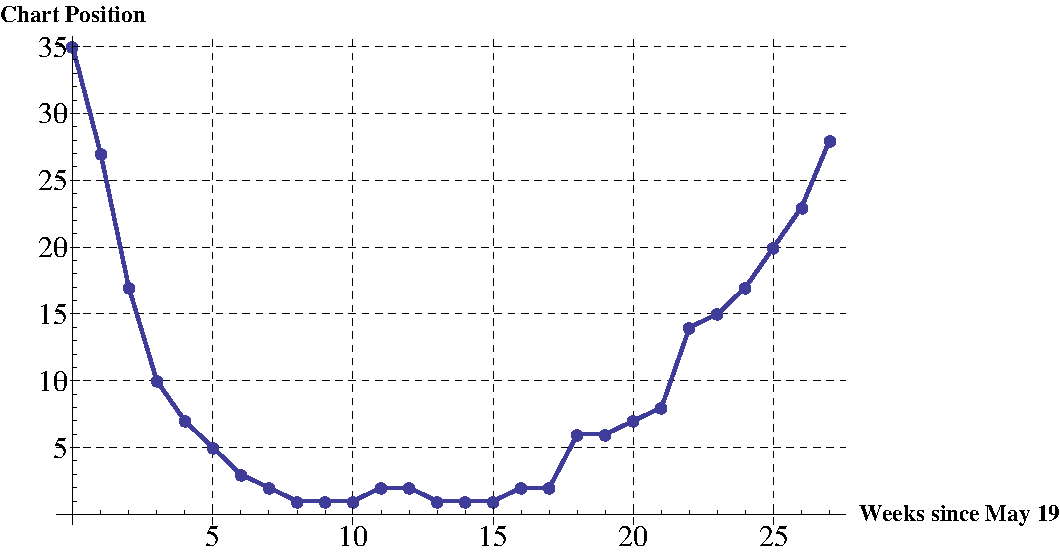
\includegraphics [width = 6in] {bigGirls}

\begin{enumerate}
\item After five weeks on the chart, what was the approximate ranking of the song?
\vfill
\item For approximately how long was the song ranked in the top ten?
\vfill
\end{enumerate}

\newpage

%%% old 1.4, sports, fun
\item At Beijing 2008, Kara Goucher (a Duluth, MN native) placed 9th in the women's 5000 meter race at a time of 15.82 minutes.

\begin{enumerate}
\item Convert 15.82 minutes into minutes and seconds.
\vfill
\vfill
\item Her speed was approximately 316 meters/minute, as you can check.  How fast is that in miles per hour?  \emph{Use 1 meter = 3.28 feet and 1 mile = 5,280 feet.}
\vfill
\vfill
\vfill
\end{enumerate}

\end{enumerate}

\end{document}
